\documentclass[12pt]{ociamthesis}
%load any additional packages
\usepackage{amsmath}
\usepackage{amssymb}
\usepackage{ltablex}
\usepackage{caption}
%\usepackage{subcaption}
%\usepackage{svg}
\setlength{\parindent}{0pt}

\newcommand*{\captionsource}[2]{%
  \caption[{#1}]{%
    #1%
    \\\hspace{\linewidth}%
    \textbf{Source:} #2%
  }%
}

\usepackage{hyperref}
% \usepackage{biblatex}
\usepackage[round]{natbib}
\usepackage[utf8]{inputenc}

\title{Predictive Computational Models\\[1ex]     %your thesis title,
        of Task Switching}   %note \\[1ex] is a line break in the title

\author{Abdel Wahab Turkmani}             %your name
\college{Oriel College}  %your college
\degree{Master of Science}     %the degree
\degreedate{Trinity 2017}         %the degree date

%end the preamble and start the document
\begin{document}

%this baselineskip gives sufficient line spacing for an examiner to easily
%markup the thesis with comments
\baselineskip=18pt plus1pt

%set the number of sectioning levels that get number and appear in the contents
\setcounter{secnumdepth}{6}
\setcounter{tocdepth}{6}

\maketitle                  % create a title page from the preamble info
\begin{dedication}
This thesis is dedicated to\\
 my friends, family and to LIFE\\
for their endless support without which\\
this degree would not have been possible
\end{dedication}        % include a dedication.tex file
\include{acknowledgements}  % include an acknowledgements.tex file
\include{abstract}          % include the abstract

\begin{romanpages}          % start roman page numbering
\tableofcontents            % generate and include a table of contents
\listoffigures              % generate and include a list of figures
\end{romanpages}            % end roman page numbering

%now include the files of latex for each of the chapters etc
 \chapter{Introduction} \label{intro}
 \section{Background}
 Traditional models of economics, psychology, and other sciences assume rational models of agents. Individuals in the real world, however, rely on heuristics with biases which appear to result in temporally inconsistent choices, false beliefs, and seemingly suboptimal planning \citep{Kahneman1979}. Often, humans make choices that change over time, do not serve their self-interest, and conflict with their stated preferences. \\

 An important application of machine learning and probabilistic programming is to essentially understand the underlying cognitive processes that characterize and explain these seemingly `sub-optimal' choices \citep{Evans2015}. The need to understand the latent factors influencing these choices has spurred research in economics, psychology, and marketing, with substantial work done on modeling and predicting future human behavior based on past behavior and certain latent factors. As machine learning and AI continue to find applicability in automating personal tasks and in interacting with people, it becomes important that these models are able to understand the nuances in human choices to better predict future behavior. To this end, developing probabilistic models of future choices based on past behavior has become a topical and important problem.\\

 Research in economics and marketing has led to several computational models that attempt to model human behavior from their exhibited choices \citep{Szenberg2009}, however, these models haven't stemmed from psychological models of human choice. Concurrently, several psychological models of human choice exist, however, these haven't been applied to the problem of behavioral model inference from observed choices \citep{Busemeyer2005, Train2003, shenoy2013rational}. Alternatively, computational models in Inverse Reinforcement Learning \citep{ng2000algorithms} and Bayesian Inverse Planning \citep{baker2009action} attempt to infer preferences by inverting a rational decision-making model based on a utility function \citep{russell1995modern}. These models, however, haven't been able to capture the full spectrum of the seeming irrationalities underlying human decision models. Their shortcomings, traditionally, have stemmed from ignoring the latent factors spurring the bounded rationality, usually by modeling these inconsistencies as noise \citep{Kim2014, Zheng2014}.\\ 

 Recent developments \citep{Evans2015, Jern2017} have attempted to correct these simplifications by explicitly accounting for the biases and heuristics developed in psychological models of human choice \citep{Kahneman1979}. Progress on this frontier has included structural modifications to the utility functions that incorporate the biases and heuristics. For example, hyperbolic discounting \citep{ainslie2001breakdown} is used to capture the tendency for temporally inconsistent choices  while uncertainty and false beliefs affecting choices are modeled through probability distributions over knowledge of the state of the world, instead of assuming agents fully know the current state of the world \citep{baker2014modeling}.\\

 Despite the success in explaining inconsistencies in choices as compared to human explanations, there remains substantial work to be done on defining expressive and representative computational frameworks. These frameworks need to be expressive and reliable enough to help AI, and human researchers, better understand human behavior. 

 \section{Motivation}
 With the proliferation of connected devices like smartphones and wearable technology, in tandem with the continued expansion and domination of the web by the attention economy, the digital world has become ever more addictive. When put to the question, experts' prediction on the future generations comes in at a gloomy conclusion: with the exception of the few capable of retaining attention and focus, many participants in the digital economy will succumb to the continuous distractions awarded by addictive, rewarding applications \citep{anderson2012millennials}. While the benefits of using the internet to support and inform our daily decisions in a hyperconnected world where access to, and verification of, information is unprecedented are largely positive, the experts surveyed in the Pew report predict that teenagers will face difficulties originating from the growing dependence and thirst for instant gratification awarded by social media and made profitable by the attention economy.\\

 The report further surveys these experts about what they consider the most desirable skills for people in 2020, and the ability to concentrate, amongst others, was emphasized. Tiffany Shalin, founder of the Webby Awards and director of \textit{Connected} remarks that a large divide lies between participants in the digital economy that develop the ability to properly allocate attention in this new environment and those that do not, with the reward being successfully navigating and participating in this hyperconnected environment.\\

 Coupled with the rapid advance of machine intelligence and personal assistants that take on more attention-intensive tasks, argues John Smart in the report, the productivity and desire of the young generation to work will be affected, with the result being the increasing willingness to be distracted and consumed by the desire for instant gratification.  With human productivity at risk, it comes as no surprise that a market has emerged for attention-aware assistants. Many applications promising to help maintain and improve attention have flooded the market in response. Some, like RescueTime, offer the ability to track usage statistics, while others take more hard-line approaches like blocking distracting applications and websites and/or offering rewards and punishments to users \citep{Lyngs}.

 The potential implications of attention-aware computational models are far-reaching. For example, models capable of predicting whether a person will switch from the required task at hand could find usage in predicting when drivers will become distracted by their devices or when a student writing his thesis will switch to binge watching movies. Models with such capabilities can then alert the driver or take action, potentially avoiding life-threatening accidents. Moreover, in an attention economy \citep{davenport2013attention} where many users report reduced productivity due to constant distractions, such models could be used in anti-distraction applications that aim to improve productivity by ensuring people remain focused on their primary tasks. With effects ranging from fatal catastrophes to reduced productivity, applications that help maximize attention have a role to play in the digital economy. Among many other functions, these applications should be able to understand the latent cognitive state people are in by observing their app-usage behaviour, and make predictions on what their future activities will look like. To better help people focus and maintain attention, it is important to be able to understand the behaviour patterns of users and differentiate between temporary interruptions and distractions \citep{Lyngs}. For example, advice on future action given to a user when they utilize an Instant Messaging application should be different when the user will likely quickly respond to the message and return to their primary task versus when their current behaviour, based on past experiences, suggest they are likely to become fully distracted and abandon the task they should be focusing on. 

 To this end, this thesis project will attempt to develop a set of models that are able to achieve two things: first, understand and generate the latent cognitive space within which people operate. By capturing these states and understanding how users use their applications we will be better able to understand the extract the heuristics that guide a users behaviour and attention models. Second, these models should be able to predict what future applications a user will likely resort to. By developing models that offer these predictive capabilities, attention management applications will be better able to guide users in increasing their productivity. The occasional break to use social media may not be bad, and may even be beneficial if it means the user will resume working; potentially more effectively due to the break. However, getting consumed by the different apps vying for a users attention, which may ultimately lead the user to abandoning the task at hand is negative, and attention-management applications would benefit tremendously from the ability to predict this. Moreover, by analyzing the predictions of these computational models and their accuracy, we can further learn more about the characteristics and properties of the latent factors affecting task-switching behavior, allowing us to improve our existing knowledge on human attention. These high-impact ramifications serve to motivate the design and analysis of such predictive models.\\

 \section{Proposed Approach}

 Several approaches exist to model attention, such as models of optimal information gain \citep{pirolli1999information}, drive and multi-tasking where people are working on several tasks and jointly trying to address them all. These approaches attempt to explain why and when we switch tasks by modelling attention directly. However, for my project, I intend to frame attention management as a problem of sequential decision making. Under this assumption, human attention involves `choices' on which current task at hand to focus on. Distractions, temptations and temporal inconsistencies influence agents when choosing which tasks to focus on. When viewed as such, the process of switching tasks can then be framed as one of sequential decision making where attention models are subject to decision and choice theory. As such, these `choices' are made based on heuristics and influenced by our internal cognitive states. The `choice' of whether to continue focusing on the current task at hand or to switch to another task is subject to several latent factors. For example, switching from the current task of work to leisure (e.g. social media) could mean the agent is done with their work, but could alternatively be due to distractions or fatigue.\\

 In approaching the task of modelling attention this thesis will focus on two distinct tasks:

 \begin{itemize}
     \item Uncovering the latent generative space of a user's app-usage behaviour
     \item Predicting how a user will spend their time across their different applications.
 \end{itemize}

 To model the latent generative space, and make predictions about future app-usage, the models will abstract away from attempting to manually devise and encode the set of heuristics agents use in deciding which app to use next. Instead, it is assumed that the heuristics employed can be captured through the patterns displayed in app-usage behaviour. To illustrate let us consider the example of a day in the life of a student. Consider a person working on her thesis. Upon waking she may check her social media feeds before meditating and having breakfast. In choosing which social media apps to use, our student may employ some heuristics. An example would be check channels that allow her to get a quick summary of global news, and consequently she uses Twitter. For meditating, our student may use the app Headspace, and choose to have one or two sessions depending on what her previous experience has led her to believe is most optimal regarding benefit vs time-spent not working on her thesis. Next, she may work until noon, where she has lunch. It is possible that our example student enjoys watching a few shows on Netflix while she eats. The number of shows she watches depends on the type of show and a myriad of heuristics she's developed over time that fit within the current context. Her day proceeds similarly where at each point in time she makes choices on what apps to use based on rules-of-thumb she's subconsciously developed over time. Ultimately, the underlying heuristics express themselves through the pattern of app-usage behaviour displayed over time. \\

 Essentially, this thesis makes the assumption that models of human task-switching and attention, along with the heuristics that guide them, can be developed using only previous observations on said individuals app-usage behaviour. To test this hypothesis, this thesis builds out a set of models that are trained on data collected by logging a user's app-usage across their devices. The models will be trained with the objective of predicting future app-usage behaviour given the data and uncovering the discussed latent space. These models will be trained on a real-life dataset of tasks attended to by people obtained from RescueTime, an application that tracks a users active applications on their devices. The logged data by RescueTime will be collected and processed into time-series data depicting the tasks the participant attended to. The input to the models will be only the labeled time-series data of tasks the agent is focusing on. As such, low-level factors such as lighting, location, mental/physical well-being, etc of the agents will be ignored. The task will strictly be to predict task-switching based on information logged by RescueTime (e.g. time of day, time elapsed since activity started, hours spent working during that day, etc). The class of predictive models will be assessed via quantitatively measuring their accuracy in predicting future app-usage behaviour. The effectiveness of the generative models in uncovering the latent space will be visualised and assessed qualitatively.

 In essence, this project will attempt to explore three questions:

 \begin{itemize}
     \item Can human attention be modeled as a sequential decision making problem and consequently captured by sequential models?
     \item Can the underlying latent states influencing the observed behaviour be learned?
     \item Does accounting for these underlying latent states help improve predictive capabilities?
 \end{itemize}


 \section{Structure of Thesis}
 % The rest of the thesis is structured as follows: First, in Chapter \ref{data} we present RescueTime, the app-activity logger and discuss it's features and limitations. An overview of how the data is collected and processed is also presented. In Chapter \ref{predmod} a class of sequential models capable of capturing the temporal dependencies in the data will be explored. The background of these models will be introduced, their contemporary applications and where they've been successful will also be briefly covered. A detailed description of the theory of these models will be presented followed by a justification of why they are chosen for this modeling task. Next, in Chapter \ref{genmod} a class of generative models that are capable of inferring generative latent spaces will be similarly explored, with a discussion on their theoretical underpinning, contemporary success and applicability to the defined problem similarly examined. Following these two chapters, in Chapter \ref{genpredmod} we discuss the recent attempts made in merging these two classes of models, and present an implementation for combining them for our purposes. in Chapter \ref{res} we present the findings of this thesis and discuss their implications and validity. Chapter \ref{conc} concludes this paper, summarising the contributions and findings of this thesis and exploring future directions of research.
\chapter{Data Collection \& Processing} \label{data}
\section{RescueTime}
RescueTime is an app available on the Android Playstore, and available for download on the Windows and MacOS platforms. It synchronizes and tracks data about applications active across the user's devices it is installed on. RescueTime collects data at the application and website level, and offer the ability to categorize a wide array of apps and websites into predefined mainstream application categories like Instant Message, General Social Networking, General Software Development, and others. A current limitation of the RescueTime platform is the granularity of data collection. Currently, RescueTime aggregates data into 5-minute buckets on local devices before storing them on the server. Consequently, the available data provides information on how many seconds an application was used in a 5-minute interval, across all apps used in that same interval. While different apps are logged within the 5-minute block, no information is available on the sequence of usage of those apps in that block. A sample of the raw data from RescueTime is displayed in Table \ref{dirtydata}. The next section discusses the data cleaning and processing performed prior to any modeling.

\begin{table}
\centering
\caption{RescueTime Data Before Processing}
\label{dirtydata}
\begin{tabular}{llll}
\hline
\{\} &                 Date & Time Spent (seconds) &                     Category \\
\hline
15 &  2017-03-01T16:10:00 &                [107] &            [Instant Message] \\
20 &  2017-03-01T16:55:00 &                 [20] &                      [other] \\
21 &  2017-03-01T16:55:00 &                  [5] &                     [Search] \\
22 &  2017-03-01T17:10:00 &                [136] &     [General News \& Opinion] \\
53 &  2017-03-01T21:55:00 &                [174] &  [General Social Networking] \\
54 &  2017-03-01T21:55:00 &                 [19] &                     [Search] \\
55 &  2017-03-01T21:55:00 &                 [14] &            [Instant Message] \\
56 &  2017-03-01T21:55:00 &                  [2] &                      [other] \\

\hline
\end{tabular}
\end{table}

\section{Data Processing}
\subsection{Categories vs applications/websites}
RescueTime collects data at the application and website level, giving us data on every application and website used over the 5-minute interval. Despite the benefits of more granular data, the data at this granularity poses several problems:
\begin{itemize}
    \item The same app, used via different channels, counts as a different app. For example, Whatsapp messenger used on the mobile app, the desktop app or the web app will count as three different 'apps' used, whereas in fact the user was engaging in the same activity.
    \item Tracking the individual websites a user accesses for a specific task results in a data explosion. For example, a user may engage several websites, such as StackOverflow, Stackshare, Github, etc when searching for solutions to a particular technical problem. With enough data collected across a large number of users, this may not be a problem. However, in this particular case, the dataset used is for only one person over a period of 6 months and such high-dimensional data may prove cumbersome to train on given the dataset size.
    \item A specific user would use a unique set of apps for an activity, while another user may use a different set of apps for the same activity. For example, one person may use PyCharm as their prefered development platform, while another may prefer using Jupyter Notebooks. Moreover, the same user may utilize several apps while doing the same activity, like using both PyCharm and Jupyter Notebooks when developing in Python. Given a large enough dataset across a number of users, it may be possible to train a model that learns the similarities and differences across apps, however given the sample and dataset size, once again, this would be cumbersome.
\end{itemize}

For the reasons detailed above, for this project only the category level data is considered, i.e. the data collected is aggregated into high-level categories pre-defined by RescueTime.

\subsection{Cleaning the data}

\subsubsection{Reducing dimensionality}
In processing the data, first we observe that only a few apps consume the majority of a users time. Figure \ref{time_spent} shows the cumulative time spent for the 25 categories that consume the most time. Empirically, we observe that only the 14 most popular apps consume 90\% of the user's recorded time.\\

\begin{figure}[htbp]
 \centering
 \caption{CDF of time-spent across most popular apps}
 \label{time_spent}
 \includegraphics[width=1\textwidth]{images/time_spent}
\end{figure}

To reduce the dimensionality of the data at each timestep, we retain only these 14 categories and lump all other categories into a generic 'other' category. Let $\mathcal{P} \in \mathcal{R}^\mathcal{D}$ denote this list of 15 categories sorted in decreasing order of total time consumed ($\mathcal{D} = 15$). These categories are visualized in Figure \ref{TimeSpentDistribution}.\\

\begin{figure}[htbp]
 \centering
 \caption{Percent of total time spent in each category}
 \label{TimeSpentDistribution}
 \includegraphics[width=1\textwidth]{images/TimeSpentDistribution}
\end{figure}

\subsubsection{Grouping timestamps} \label{group_t}
Moreover, the data from RescueTime is formatted such that for a single timestamp, a different datapoint exists for each app used in that block as can be seen in the last four rows in Table \ref{dirtydata}. For the same timestamp, 2017-03-01T21:55:00 we have four rows that each show a different category. During pre-processing, these data points are aggregated into a vector of size $\mathcal{D}$.
where each index contains the time spent on the corresponding application, with the order following that of $\mathcal{P}$. As an example, the last four rows would be grouped together into a single timestamp with entry, called the Activity Vector $x$, $x = [14,0,0,174,0,0,0,0,19,0,0,0,0,0,2]$. Each entry in an Activity Vector represents the number of seconds spent on apps in the corresponding category defined in $\mathcal{P}$ across a 5-minute, or 300-second, interval. To normalize the Activity Vectors to the range $[0,1]$ we divide all entries by 300. It is worth noting that the sum of time spent on all categories in each 5-minute block need not equal 300 seconds as it is possible a user does not utilize their devices/apps for the entirety of the 5-minute interval.

\subsubsection{Missing data}
As alluded to in \ref{group_t}, RescueTime collects no data when apps are not being used. Consequently, in 5-minute intervals where no apps are used on any device, for example when sleeping or just generally not using ones devices, RescueTime reports no entry for that interval. These datapoints however need to be included, as using no applications on any device still contains information about a user's app-usage behaviour. To fill in these data points, we expand the dataset to contain all 5-minute blocks over the collection period and fill the missing entries with an Activity Vector of zeros indicating that in the specified time-interval no applications were used. A sample of the final cleaned data is shown in Table \ref{cleandata}


\begin{table}
\centering
\caption{RescueTime Data After Processing}
\label{cleandata}
\begin{tabular}{ll}
\hline
Date  &                       Activity Vector \\
\hline
2017-03-01T00:00:00 &  [0.133333333333, 0.0, 0.0, 0.0, 0.0, 0.0, 0.0,... \\
2017-03-01T15:20:00 &  [0.0366666666667, 0.0, 0.0, 0.0, 0.0, 0.0, 0.0... \\
2017-03-01T17:10:00 &  [0.133333333333, 0.0, 0.0, 0.0, 0.0, 0.0, 0.0,... \\
2017-03-01T17:15:00 &  [0.0, 0.0, 0.0, 0.0, 0.0, 0.0, 0.0, 0.0, 0.0, ... \\
2017-03-01T17:20:00 &  [0.0, 0.0, 0.0, 0.0, 0.0, 0.0, 0.0, 0.0, 0.0, ... \\
2017-03-01T17:45:00 &  [0.07, 0.0, 0.0, 0.0, 0.0, 0.0, 0.0, 0.0, 0.0,... \\
2017-03-01T17:55:00 &  [0.0, 0.0, 0.0, 0.16, 0.0, 0.0, 0.0, 0.0, 0.01... \\
2017-03-01T18:00:00 &  [0.0, 0.0, 0.0, 0.0333333333333, 0.0, 0.0, 0.0... \\
2017-03-01T19:00:00 &  [0.02, 0.0, 0.0, 0.0, 0.0, 0.0, 0.0, 0.2866666... \\
2017-03-01T19:35:00 &  [0.0733333333333, 0.0, 0.0, 0.0, 0.0, 0.0, 0.0... \\
2017-03-01T19:55:00 &  [0.03, 0.0, 0.0, 0.0, 0.0, 0.0, 0.0, 0.0, 0.02... \\
2017-03-02T17:55:00 &  [0.0, 0.0, 0.0, 0.0166666666667, 0.0, 0.0, 0.1... \\
\hline
\end{tabular}
\end{table}
 \chapter{Background} \label{bg}
 \section{Supervised and Unsupervised learning}
 While the models and applications of machine learning are numerous and cover many varied domains and problems, at a fundamental level, machine learning addresses three classes of problems: the problem of uncovering a mapping from an input to an output, learning how policies through experience, and the problem of uncovering interesting and meaningful structure and patterns in a dataset. The first class of problems are commonly referred to as that of Supervised Learning, the second as Reinforcement Learning, and the latter as Unsupervised Learning. For the rest of this thesis, we will mainly concern ourselves with the areas of Supervised and Unsupervised Learning.\\

 In the Supervised Learning setting, models are trained to uncover a mapping $y=f(x)$ between inputs $\mathbf{x}$ and outputs $\mathbf{y}$ in a dataset $\{\mathbf{x}_i, \mathbf{y}_i\} | i=1.. \mathcal{D}$. The source of inputs vary widely, ranging from images to medical information to natural language, with the outputs following a similar pattern. To encode these different sources of inputs and outputs, the inputs and outputs take on mainly two different types: real-valued vectors or nominal/categorical vectors, i.e. $\mathbf{x} \in \mathcal{R}^N$ or $\mathbf{x} \in \{0,1\}^N$ with the same holding for y. For the cases where $y \in \mathcal{R}$, the supervised learning model learns to predict continuous valued outputs, and the task is termed \textit{regression}. The other case, where $\mathbf{y} \in \{0,1\}^N$ the model is trained to predict categorical/binary outputs and the problem is termed \textit{classification}. In the classification task, the model is trained to classify an input $\mathbf{x}$ into one of $N$ possible classes, for example, given medical information about a patient, classify whether the patient has the flu or not. In the regression instance the model is trained to predict a continuous value given the input $x$, for example, given information about a house and its surrounding area predict the price of the house.\\

 In the Unsupervised Learning setting, models are trained to discover interesting patterns inherent in the data. The dataset $\mathbf{x}_i | i=1..\mathcal{D}$ has no label to be classified into or forecasted, and these types of problems tend to be more complicated since they are less well defined \citep{murphy2012machine}. Examples applications of Unsupervised Learning include clustering, topic modelling, generative models, etc.

 \begin{figure}
     \centering
     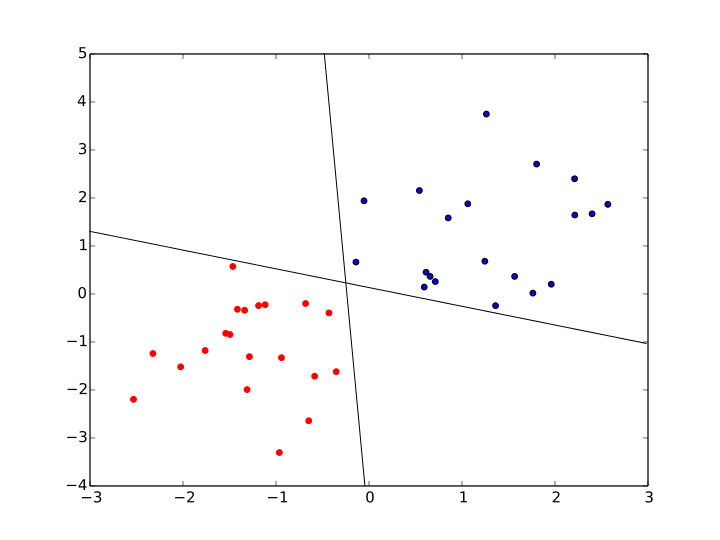
\includegraphics[width=.5\textwidth]{images/KnnClassification}
     \caption{(a) Classification Problem}
     \label{fig:classification}
\end{figure}%

\begin{figure}
     \centering
     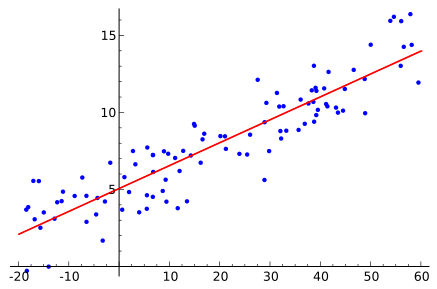
\includegraphics[width=0.5\textwidth]{images/Linear_regression}
     \caption{(b) Regression Problem, \cite{reg}}
     \label{fig:regression}
 \end{figure}


 \citep{murphy2012machine}
 \section{Neural Networks}
 Central to many of the recent advances in machine and deep learning is the perceptron. The perceptron serves as the building block of neural networks and all the consequent derivatives such as convolutional and recurrent neural networks. The perceptron takes a vector of real-valued or ordinal inputs $\mathbf{x_i}$, multiplies each by a weight $\mathbf{W_i}$, applies an activation function $\phi$ to generate an output $y_i$. Formulated mathematically, the perceptron behaves as follows:

 \begin{equation}
     y_i = \phi ( \sum_{j=1}^n w_{ij} x_i) 
 \end{equation}

 where $\phi$ represents the activation function which could be a linear or, more commonly, a non-linear function such as the logistic sigmoid, $\frac{1}{1+e^{-x}}$, the hyperbolic tangent, $\frac{e^{2x} -1}{e^{2x} + 1}$, or the more recently popular rectified linear units \citep{nair2010rectified} $f(x) = max(0,x)$ and exponential linear units \citep{clevert2015fast}, $f(x) = x * (x > 0) + (x < 0) * (\alpha * (e^x - 1))$. The choice of these activation functions is often problem dependent, and has a substantial effect on accuracy and training time. Usually, these activation functions are also increasing, continuous, bounded and differentiable.

 When many of these neurons are stacked we have a layer of neurons, more commonly known as an Artificial Neural Network. Information in the ANN moves forward, from the inputs through the layer of neurons, known as the hidden layer, to the output. By including more neurons in the hidden layer and utilising non-linear activations, the ANN becomes a powerful function approximator that can be efficiently trained to recover functions that map inputs to outputs \cite{murphy2012machine}. ANNs with many hidden layers between the input and output are known as deep neural networks and they are responsible for many state-of-the-art results across the three main areas of machine learning.

 \section{Recurrent neural networks}
 Recurrent neural networks are, at the most fundamental level, neural networks with loops. These loops allow information to persist through time by repeatedly including previous information, stored in a hidden state, in the computations at each time-step. At each time-step, the RNN computes a hidden state h, which can be used to make a prediction on the next element in the sequence. In applications with discrete observations such as language modelling, the prediction at each time-step would be a distribution over a set of possible outcomes, in this case words or characters, given the previous elements in the sequence. Alternatively, RNNs can be trained to predict a single real valued number, or multiple values in a multi-variate time-series forecasting problem such as ours. More rigorously, the RNN models time-series data and makes predictions via the following equations:

 \begin{equation}
     h_n = f(x_n, h_n-1) = g_1(\mathbf{V}_xx_n + \mathbf{V}_hh_{n-1} + \mathbf{c})
 \end{equation}

 \begin{equation}
     y_{out} = f(h_n) = g_2(\mathbf{W}h_n + \mathbf{b})
 \end{equation}

 Where $g_1$ is the activation function applied to every element in the hidden state, and $g_2$ is the activation function applied at the output. The activation at the output could be a softmax for prediction a distribution across a discrete set of outputs, or for continuous regression the logistic sigmoid, the hyperbolic tangent, the popular ReLu \citep{nair2010rectified}, their recent variants the eLu \citep{clevert2015fast} that have been shown to speed up training, or nothing at all. \\

 \begin{figure}
     \centering
     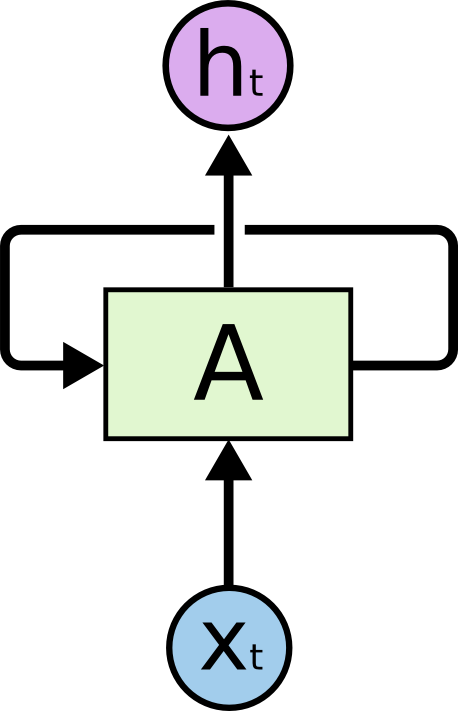
\includegraphics[width=0.2\textwidth]{images/RNN-rolled.png}
     \caption{Rolled RNN, image from http://colah.github.io/posts/2015-08-Understanding-LSTMs/}
     \label{rolled_rnn}
 \end{figure}

 While theoretically RNNs are able to capture information infinitely far in the past, in practice RNNs are 'unrolled' for a finite number of timesteps into the past, over which they are allowed to learn the temporal dependencies. 

 \begin{figure}
     \centering
     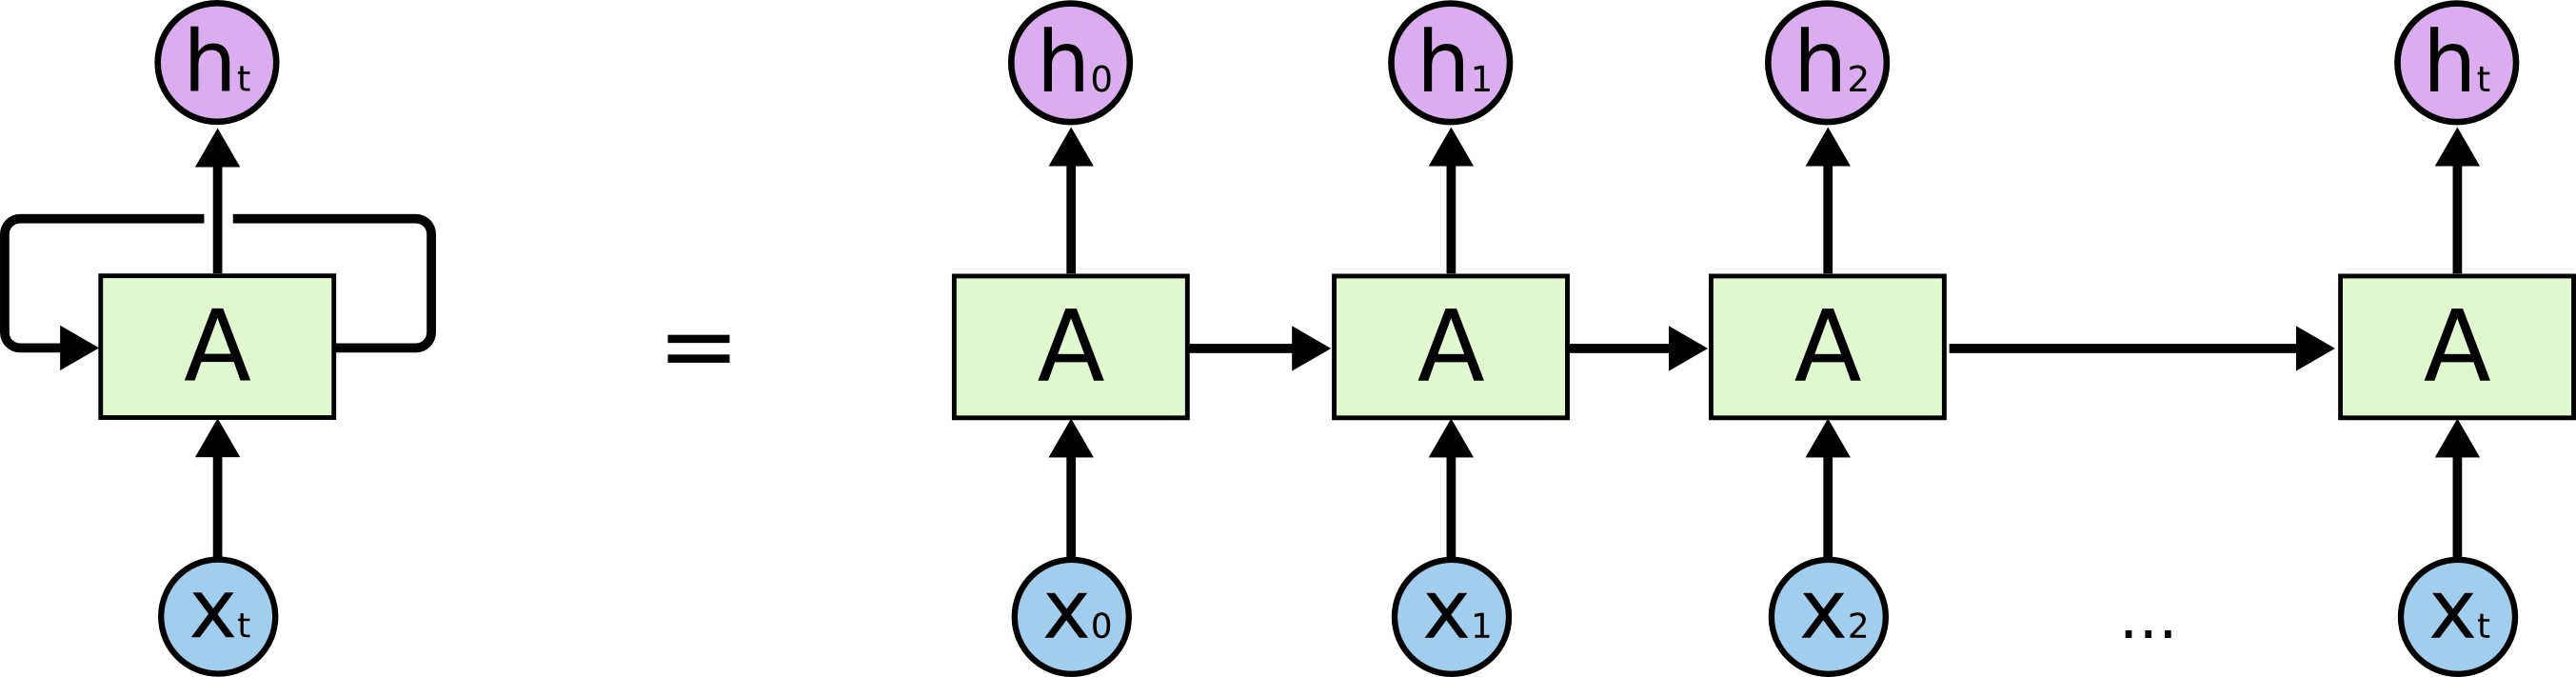
\includegraphics[width=1\textwidth]{images/RNN-unrolled.png}
     \caption{Unrolled RNN, image from http://colah.github.io/posts/2015-08-Understanding-LSTMs/}
     \label{unrolled_rnn}
 \end{figure}

 When unrolled over time and trained to capture dependencies that span over long-ranges, RNNs begin facing the problem of vanishing gradients where the propagation of gradients backwards through time may result in consecutively multiplying many gradients smaller than 1 with each other, such that eventually the gradient approaches 0.\\

 To remedy this, the LSTM \citep{Hochreiter1997} and GRU \citep{Cho2014} have been proposed. These cells overcome the vanishing gradient by introducing two properties, gating and memory. Through gating, these cells are able to propagate gradients backwards essentially through addition thereby circumventing the consecutive multiplication of gradients. Memory cells on the other hand improve the ability to learn long-term dependencies by allowing the LSTM cells to store information in these memory cells, using and overwriting them when needed. In what follows we use an LSTM that implements input, output and forget gates to build its memory cell. These gates respectively allow information into the cell, out of the cell, and cause the LSTM to forget what is stored in memory. Once again, $\mathbf{h}_n$ represents the hidden state of the LSTM cell.

 \begin{equation}
     \begin{split}
         & \mathbf{i}_n  = \sigma(\mathbf{W}_i [\mathbf{x}_{n-1}; \mathbf{h}_{n-1}; \mathbf{c}_{n-1}] + \mathbf{b}_i) \\
         & \mathbf{f}_n  = \sigma(\mathbf{W}_f [\mathbf{x}_{n-1}; \mathbf{h}_{n-1}; \mathbf{c}_{n-1}] + \mathbf{b}_f) \\
         & \mathbf{o}_n  = \sigma(\mathbf{W}_o [\mathbf{x}_{n-1}; \mathbf{h}_{n-1}; \mathbf{c}_{n-1}] + \mathbf{b}_o) \\
         & \mathbf{c}_n =  \mathbf{f}_n \odot \mathbf{c}_{n-1} +  \mathbf{i}_n \odot \mathrm{tanh}(\mathbf{W}_c [\mathbf{x}_{n-1}; \mathbf{h}_{n-1}; \mathbf{c}_{n-1}] + \mathbf{b}_c) \\
         & \mathbf{h}_n =  \mathbf{o}_n \odot \mathrm{tanh}(\mathbf{c}_n)
     \end{split}
 \end{equation}

 \section{Convolutional Neural Networks}
 Convolutional Neural Networks are variants of Vanilla Neural Networks that address the problem of training deep fully connected networks. Convolutional Neural Networks reduce the number of parameters to be learned in a densely connected network by imposing restrictions on the number of neurons in a previous layer any neuron can be connected to \citep{gamboa2017deep}. Groups of neurons, called convolutional filters, share the same weights and process different portions of the input. These filters are convolved with portions of the input, in either 1 or 2 dimensions. The convolutional filters can be convolved with the input to the CNN along any number of dimensions to extract features along those dimensions. For example, a 2D convolutional filter will be convolved with an input image to extract features along both dimensions of an image whereas in the case of input data such as time-series, a 1D convolutional filter can be used and convolved along one dimension, time, to extract temporally relevant features.
\chapter{Variational Autoencoder} \label{genmod}
\section{Introducing the problem}



\section{Generative Models Overview}

Generative models are a class of machine learning algorithms that aim to learn distributions $P(X)$ over a dataset $X | x \in \mathcal{R}^\mathcal{D}$. The class of generative models approach pattern recognition in line with Feynman's "what I cannot create I do not understand". Given a point $x \in X$ a generative model will try to uncover the patterns existing in $x$'s structure, i.e. between the parts that comprise $x$, and often, this learnt space that describes the patterns inherent in the structure of $X$ is low-dimensional.\\

Generative models generally fall under the umbrella of unsupervised learning, and often have applications similar to those of other traditional unsupervised learning methods such as PCA, Gaussian-Mixture-Models and Kernel Density Estimation. When tasked with uncovering a distribution $P(X)$ over a dataset $X$ these generative models can be used to uncover the density distribution over the dataset, and consequently allow us to measure things like the likelihood of points in this space, similar to GMMs and KDE. When tasked with learning a distribution $P(Z)$ that is generative of $X$ where $dim(z) < dim(x)$ then effectively these generative models learn a lesser-dimensional space that minimises some measure of reconstruction error, similar to PCA and Kernel-PCA.\\

Beyond learning distributions $P(X)$ and $P(Z)$ over the dataset, generative models also allow us to sample points from the learned distribution. For example, by learning a distribution over a dataset of images of trees, a generative model will allow us to sample new images of trees from the distribution that look very much like the images in our database, but aren't exactly like the images we already have. One can imagine the applications of this in graphic design and video production! Training models that allow us to generate completely new samples from the learned distribution have been explored for quite some time in the machine learning community, however until recently they have all faced one of three problems: they make strong assumptions about the structure in the data, and when these assumptions do not hold, they make sub-optimal approximations that fail to comprehensively learn generative distributions. When the models succumb to neither of these shortcomings, they often rely on very expensive inference techniques like Markov Chain Monte Carlo \citep{doersch2016tutorial}.\\

Recently, two new classes of generative models have emerged that address all three of these problems: Generative Adversarial Networks \citep{goodfellow2014generative} and the Variational Autoencoder \citep{kingma2013auto}. Generative Adversarial Networks operate within the framework of finding a Nash Equilibrium between a generator network, $G$ that learns the distribution $P(X)$ and a discriminator network $D$ that attempts to classify whether the points generated by $G$ do come from the space inhabited by the data points. Variational Autoencoders on the other hand have sprung out from the merger of Bayesian inference with Machine Learning, particularly the Autoencoder. In this chapter, we will explore the Variational Autoencoder and its application to estimating a distribution over our dataset, and in the process uncovering the structure and patterns in the way user's truly use their applications.


\section{Variational Autoencoder}
\subsection{Autoencoder}
Traditional Autoencoders behave like compression-decompression algorithms in that they take high dimensional data and embed them into a low dimensional space, and from that space they attempt to reconstruct the original input. In doing so, Autoencoders are trained to minimize the reconstruction error by finding a hidden representation that accounts for as much of the variance as possible. In that sense, they behave most similarly to PCA. The process of training a model that learns this encoding-decoding process is normally known as representation learning. The benefits of these models normally stem from the myriad ways these low-dimensional representations can be used. For example, they can be used to learn similarities between objects based on distances in this lower dimensional space, for use in NLP systems in semantic embedding, or for reducing the dimensionality of inputs to other models.

 \begin{figure}[htbp]
     \centering
     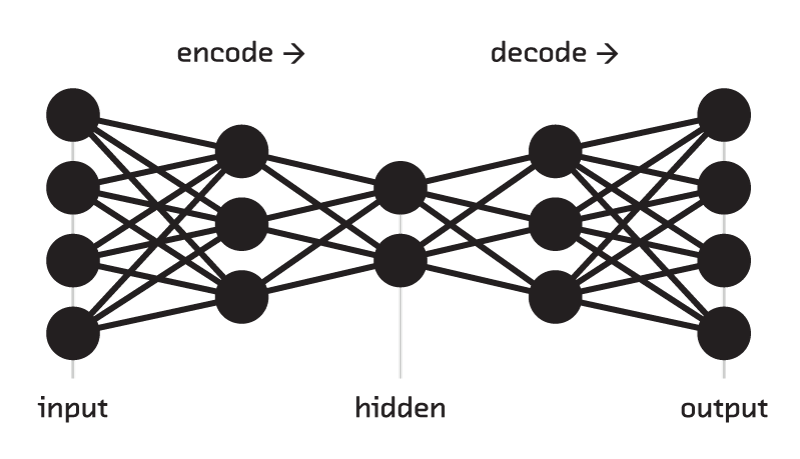
\includegraphics[width=1\textwidth]{images/miriams-figure.png}
     \caption{Autoencoder, \citep{_lorenz_}}
     \label{fig:ae}
 \end{figure}
 
 This process of training only on the reconstruction error often results in learning low-dimensional mappings that minimise information loss, behaving very similarly to other dimensionality reduction techniques like PCA. When trained as such, the Autoencoder consequently doesn't learn any new and interesting features about the dataset it is encoding. To remedy this, many interesting advances have been made in regularising the Autoencoder. At the cost of fidelity, regularisation, for example enforcing sparsity constraints and regularising the weights of the encoder/decoder, forces the Autoencoder to discard all but the most salient and important hidden features. The Variational Autoencoder is a form of Autoencoder that regularises the encoding-decoding process by simultaneously learning a distribution over the data and over a latent space with a designated prior.
 
\section{Variational Autoencoders}

\subsection{Intuition} \label{vae_intuition}
Consider the task of generating images of animals. When people generate images, for example by drawing or just plain imagination, we make a set of decisions before generating the image. To generate the image of a dog, we first decide what it is we wish to generate, the first obviously being that what we wish to generate is the image of a dog and not a cat. Next we might decide that the dog we wish to generate an image of is a Dalmatian. By deciding that the dog will be a Dalmatian we have implicitly made other decision about this dog: that it will be short-haired and spotted. This is an example of the dependencies present in real-world data that are not accounted for by models like Autoencoders. Next, we may decide that this dog will be quite a large dog. In doing so our image of the large Dalmatian dog is constrained by the normal proportions existent in Dalmatian dogs. We cannot have a large Dalmatian with a head the size of a pebble, or feet the size of an elephant's. These decisions illustrate a key characteristic about the process of generating realistic images of animals: before generating anything, we first make a decision about what animal we want to generate an image of. Next we decide on the properties of this animal. In order for the image to be realistic the properties we decide on must be constrained and they must respect the dependencies between different properties of the respective animal, i.e. a Dalmatian's body has certain proportions it must respect be it a large or small Dalmatian. Formally speaking, before generating an image we make a set of decisions on what latent variables our image will be generated from \citep{doersch2016tutorial}, subject to constrains on the dependence of different latent variables on each other.\\

\subsection{Theory} \label{vae_theory}
The process discussed in \ref{vae_intuition} illustrates the concept of a latent variable model. Variational Autoencoders make the assumption that an observation $x \in X$ is just the tip of the iceberg. $x$, in fact, is just a sample that is generated from $z$, a variable in a hidden/latent space $Z$.

 \begin{figure}[htbp]
     \centering
     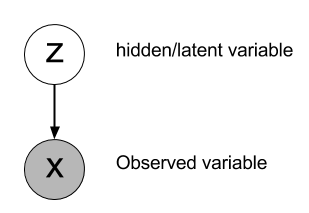
\includegraphics[width=0.5\textwidth]{images/latent.png}
     \caption{Latent variable, from \citep{eric_jang}}
     \label{fig:latent}
 \end{figure}

Given this setup, assume we have a distribution $P(z)$ over $z$ from which we can easily sample points, and that $x$ is generated by mapping a sample $z$ from the latent space to $X$ by a deterministic function $f(z;\theta)$ which is parameterised by some vector $\theta$ from another space $\Theta$. To learn a generative model we would therefore want to learn a $f(z;\theta)$ that creates $x$'s that are likely under $P(X)$. If we do learn such an $f(z;\theta)$ we expect its outputs to follow the distribution $\mathcal{N}(X|f(x;z), \sigma^2 * I$. This simply means that our function $f$ creates points that are likely to produce samples that are like $X$ and not produce samples that are not like $X$. Now, if we want to generate points that are realistic, i.e. likely, then we wish to maximise, under the generative process and training set, the probability $P(X)$. Using the law of total probability, we can set up this problem as maximising the following

\begin{equation}
    P(X) = \int P(X|z;\theta)P(z)dz
\end{equation}
where we have marginalised $z$ out of $P(X,z)$ and $P(X|z; \theta)$ replaces $f(z;\theta)$. Formulated like this, it becomes straightforward to estimate $P(X)$, all we have to do is sample points $N$ latent variables $z$ from $P(Z)$ and estimate $P(X)$ as follows:

\begin{equation}
    P(X) = \frac{1}{N} \sum_i^N P(X|z_i)
\end{equation}

To sample $z_i$'s from $P(z)$ we would need to know what the distribution of $P(z)$ is, which we don't. The VAE addresses this by observing that whatever the distribution of $P(z)$ is, if it is $d$ dimensional then it can be approximated by $d$ normally distributed random variables and a sufficiently complex function approximator, which we already have in $f(z;\theta)$! The process of generating $X = f(z; \theta)$ now becomes a two-step process where we first sample $z$ from a standard normal $\mathcal{N}(0,1)$, then mapp this sampled $z$ to the true latent, which we now rename to $\hat{z}$, from which we finally generate $X$. Normally, $f(z;\theta)$ is modelled by a sufficiently high capacity neural network to ensure it is capable of learning the mapping from $z$ to $\hat{z}$ to finally $X$.\\

Now that we have a way of sampling $z_i$, computing $\frac{1}{N} \sum_i^N P(X|z_i)$ becomes possible once again. However, given that we have defined $z_i$ to come from $\mathcal{N}(0,1)$ and observing that $P(z|X)$, the subspace of $P(z)$ that is likely to have generated $X$, is likely substantially smaller than $P(z)$ we note that in practice we would require many samples of $z_i$ for $P(X|z_i)$ to sufficiently approximate $P(X)$. The process of sampling many points from $P(z)$ results in very slow convergence is undesirable. Ideally, it would be preferable if we only sampled $z_i$'s from $P(z)$ that are likely to have generated $X$, i.e. from $P(z|X)$ however this posterior is usually intractable to compute. Instead of trying to infer this intractable posterior, the VAE performs inference on another distribution $Q(z|X)$ which is chosen to follow a distribution we know how to perform inference over, normally a Gaussian $\mathcal{N}(z|\mu_q(X), \sigma_q(X)$. The mean $\mu_q(X)$ and standard deviation $\sigma_q(X)$ are created through some deterministic sufficiently complex function approximator, for example a neural network, $g(X;\phi)$ in a similar fashion to $f(z;\theta)$. The trick is to realize that while $Q(z|X)$ is not the same as the true $P(z|X)$, if we manage to find a $Q(z|X)$ that is similar to $P(z|X)$ through, for example, mean-field approximation, then our sampled points $z_i$ would be good enough.

 \begin{figure}[htbp]
     \centering
     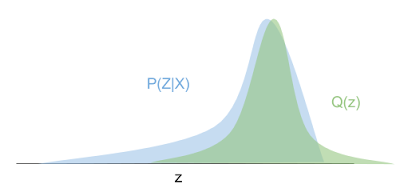
\includegraphics[width=0.5\textwidth]{images/mean-field.png}
     \caption{Q(z): a variational approximation to P(z|X) \citep{eric_jang}}
     \label{fig:mean_field}
 \end{figure}

Mean-field Variational Bayes defines the Reverse KL Divergence as an appropriate measure of dissimilarity between two distributions. To achieve a $Q(z|X)$ that resembles $P(z|X)$ we would like to minimize this KL-Divergence metric:

\begin{equation}
    KL(Q(z|X)||P(z|X)) = E[\log Q(z|X) - \log P(z|X)]
\end{equation}

By applying Bayes' rule to $P(z|X)$, and rearranging the above we arrive at:

\begin{equation} 
    KL(Q(z|X) || P(z|X)) = E[\log Q(z|X) - \log P(z)] + E[\log P(X|z)] + \log P(X)
\end{equation}

Here, we make two observations:

\begin{itemize}
    \item The term $E[\log Q(z|X) - \log P(z)]$ is nothing but the KL-Divergence between $Q(z|X)$ and $P(z)$. Given that we defined $P(z)$ to be $\mathcal{N}(0,1)$ and $Q(z|X)$ to be $\mathcal{N}(z|\mu_q(X), \sigma_q(X)$ this becomes a KL-divergence between two multi-variate Gaussians (with a k-dimensional Gaussian) which has a closed form solution:
    \begin{equation}
        KL (Q(z|X), P(z)) = \frac{1}{2} (\sum_k (\sigma_q(X) + \mu_q^2(X)^T - 1 - \log (\sigma_q(X))
    \end{equation}
    \item The term $E[\log P(X|z)]$ is the reconstruction error between generated points $X$ from our latent space $z$
\end{itemize}
 
 and, after rearranging, finally state the Variational Autoencoder Loss:
 \begin{equation}
      \log P(X) - KL(Q(z|X) || P(z|X)) =  KL (Q(z|X), P(z)) + E[\log P(X|z)]
 \end{equation}
 
 This loss function has an intuitive meaning: we learn our model's distribution $\log P(X)$ subject to some error $KL(Q(z|X) || P(z|X))$ by minimising the reconstruction loss of of our generator $\log P(X|z)$ and the divergence of the latent space produced by our encoder $Q(z|X)$ from the prior on the latent space $P(z)$. It also neatly summarises how a VAE is trained: To learn the distribution $P(X)$, the VAE's Encoder $g(X; \phi)$ learns how to transform $X$ into the latent space $z$ such that the distribution $Q(z|X)$ is as close as possible to the true $P(z)$. Next, the decoder samples points from $Q(z|X)$ and decodes them back into the original space $X$ and is trained to minimize this reconstruction error. The VAE can be trained end-to-end using Stochastic Gradient Descent (SGD) albeit for one problem: while SGD can handle stochastic inputs, it cannot backpropagate errors through stochastic variables like the sampled values of $z$. To overcome this, VAE's employ the \textit{reparameterization trick} whereby instead of sampling $z$ from $\mathcal{N}(\mu_q(X), \sigma_q(X))$ it is sampled from $\mu_q(X) + \epsilon*\sigma_q(X)$ where $\epsilon \in \mathcal{N}(0,1)$. By doing this, we can push $\epsilon$ out of the network to become a stochastic input which SGD can handle. This makes the entire network differentiable end-to-end and trainable by SGD. A schematic of the VAE is shown in Figure \ref{fig:vae_schema}.
 
 \begin{figure}[htbp]
     \centering
     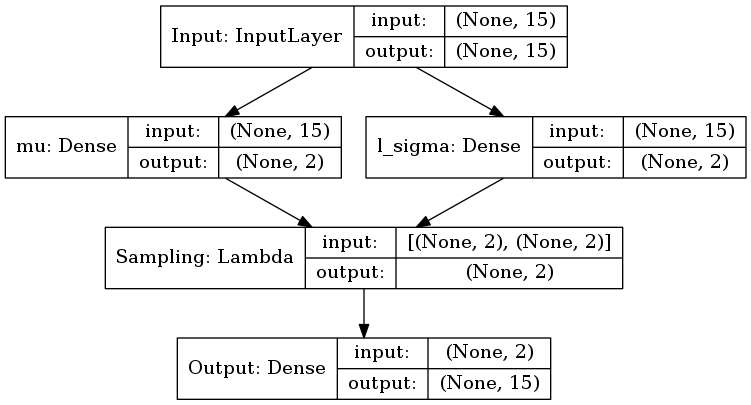
\includegraphics[width=0.5\textwidth]{images/vae}
     \caption{Schema of Variational Autoencoder}
     \label{fig:vae_schema}
 \end{figure}

\section{Implementation \& Results}
In many applications of machine learning, dimensionality reduction is performed prior to training models. By reducing the dimensionality of the input space we strive to make the learning task easier by reducing the amount of information the model has to learn about the input space. While this particularly applies to tasks where the input space is very high-dimensional that it results in very large models, that need not be the case. Often times, the input to our model can be low-dimensional but sparse, or noisy, or both at the same time. In other cases, the data might be simultaneously highly-structured and be highly varied. To give a concrete example, let us consider our own dataset of app-usage behaviour. More specifically, let us consider a particular task our user regularly engages in: Software Development. Given that our data points are aggregated points over 5-minute blocks, each 5-minute block where the user is 'focusing' on Software Development can be highly-varied. In certain cases the user might be testing their program and thus visualising a lot of the results. The user may use various different apps to visualise their results. They might also be consulting online forums and Github for support developing her program. At different times the user may be utilising any number of these different apps to perform the same task of Software Development. Even further, given the same set of apps used in different time steps, the distribution of time across these applications may vary highly as they are subject to many events which we cannot account for in our models. We can choose to consider these external factors on which the particularities depend and that we cannot model as 'noise'. \\

Given such a dataset, it may be helpful to use a dimensionality-reduction procedure that captures these main modes of operation and reduces the variance in the model. A particularly common algorithm used for this purpose is Principal Component Analysis. Alternatively, a Variational Autoencoder's encoder can be used for the same purpose and in what follows we compare the results of dimensionality reduction on our dataset between PCA and the VAE's encoder. 

\subsection{PCA Results}
Principal Component Analysis is a statistical orthogonal transformation that converts a set of observations comprising possibly correlated features in a space into a subspace where the new features are uncorrelated and explain the maximum variance in the dataset. The results are such that the first principal component explains the maximum variance in the dataset, the second component explains less than the first and so on. To visualise the results of PCA, we apply the transformation to our dataset and, for the sake of visualisation, plot the dataset against the first and second principal components:

\begin{figure}[htbp]
    \centering
    \includegraphics[width=1\textwidth]{images/PCA}
    \caption{Principal Component Analysis}
    \label{fig:pca}
\end{figure}

To describe the plot: each point represents an Activity Vector that describes the distribution of time spent across the activities in $\mathcal{P}$. Each app in $\mathcal{P}$ has a colour associated with it shown in Figure \ref{TimeSpentDistribution}. In this plot, and all plots of the dataset that follow, each point's colour is a weighted sum of the colours of each app, weighted by time spent on the respective app. For example, a point that represents a five minute block in which the user solely does 'Software Development' will have a colour corresponding to that of 'Software Development': orange. In the case where the user uses only Instant Messaging apps, the colour will be the corresponding green. If the user splits their time between these two activities, then the colour of that point will be a weighted average, or blend, between orange and green according to the time spent across the two activities. Also worth noting, the brighter a colour the more time spent on that particular app, and consequently dark points indicate points where the distribution of time across all apps in the 5-minute block does not sum up to 300 seconds. \\

As can be observed from the PCA plot, low-dimensional space into which the datapoints are projected tries to account for the maximum amount of variance in the original dataset by prioritising the apps whose usage varies the most. Intuitively, we can see this from the plot by observing that the points are clustered along 3 main axes: Video, Instant Messaging and Software Development. While some co-occurrence information is captured, for example the set of points between the two main orange and green axes that tells us Software Development and IM tend to happen together, by and large the PCA embeddings discard most of the information that does not explain variance. In datasets where certain features tend to have much larger variance than others, this is expected. Normally, such a problem would be easy to correct for by scaling the features to have the same variance, however this scaling inherently destroys the important information encoded in the scale of variance of different apps. Naturally, the way we use our different applications have unique patterns. Certain classes of apps, like Instant Messaging, are used either sparingly in a 5-minute block, or are focused on entirely and consume the entire 5-minute block. Other apps like search are mostly used sparingly in 5-minute blocks, mostly as a transition stage into other apps (Browser, General News \& Opinion, Reference \& Learning). This difference in usage pattern is an important piece of information we would not wish to discard, and is quite critical in truly understanding how a person uses their applications. This example illustrates the short-coming of PCA's emphasis on variance which make it an inappropriate tool for encoding app-usage data, summarized below:

\begin{itemize}
    \item PCA is scale-invariant and consequently penalises features that have a lesser magnitude of variance.
    \item It is possible to correct for the above by pre-scaling the features to have the same magnitude of variance.
    \item Pre-scaling however destroys the information inherent in the scale of variance across different features.
\end{itemize}

In addition to the suboptimality of encoding to maximise variance in this dataset, PCA makes the assumption $P(X)$, the density distribution over $X$ is a Gaussian distribution. This assumption may not necessarily hold in the case of our dataset, while the individual features may be normally distributed, $P(X)$ may result from a non-linear relationship between the individual components, which inherently cannot be captured by PCA. Ideally, we would like a dimensionality-reduction technique that makes a minimal set of assumptions about the form of $P(X)$, such as the VAE.


\subsection{VAE Encoder Results}
The VAE overcomes the shortcomings of the PCA through the following properties:
\begin{itemize}
    \item The VAE makes no assumptions about the form of $P(X)$. Instead it approximates it using the standard normal $Q(X)$ by minimising the Kullback-Leibler divergence between $P(X)$ and $Q(X)$. By not making any assumptions about $P(X)$ the VAE is not hamstrung by input data that is not normally distributed. In fact, to an extent, the VAE can handle input data that comes from any distribution.
    \item The VAE's loss function tries to jointly minimise the reconstruction error $\log P(X|z)$ and the KL-divergence $KL (Q(z|X), P(z))$ where $P(z)$ is our prior on the density distribution of the latent space.
\end{itemize}
The second point is particularly important in understanding the difference between the VAE's encoding process and PCA. To illustrate this, consider the regular Autoencoder (AE). An AE is also a two-stage encoder-decoder neural network that encodes input data X into a lower dimensionality space H, and decodes from H back to X. The AE is a simpler case of the VAE where there is no stochastic component (sampling) and everything is deterministic. In comparison to the VAE, the AE is trained to solely minimize the reconstruction error. Given a linear AE trained under this objective function, the linear AE will learn to approximate the optimal linear encoder - PCA \citep{Goodfellow-et-al-2016} The VAE moves beyond this by both allowing for non-linear encoders and decoders and regularising the encoding process through enforcing a normal distribution on the latent space. Consequently, during encoding we expect the VAE's encoder to move beyond encoding for maximum variance to learning a more representative encoding, i.e. latent space, of the data. 

 \begin{figure}[htbp]
     \centering
     \includegraphics[width=1\textwidth]{images/VAE_Latent_Space3}
     \caption{Latent space of the VAE's encoder}
     \label{fig:vae_latent}
 \end{figure}

By comparing the plot of the PCA encoding against that of the VAE, we observe that while both plots share a similar feature in how the data is distributed, primarily along different axes on which one particular app is concentrated, the VAE's encoder is able to assign equal important to the different apps, assigning each one a component of variance along which it is dominant. This contrasts with the PCA's encoding where only 3 major axes of variation are represented. A critical point to note is that while indeed the VAE is able to distribute importance more evenly across the different apps, the latent space is still characterised by sparsity in between the major components of variance, on which a single app is dominant. Given the normal distribution prior imposed on $P(z)$, we instead expect to see the distribution of points in the latent space, $Q(z|X)$, following the standard normal prior $\mathcal{N}(0,1)$. Moreover, from Figure \ref{fig:vae_losses} and Table \ref{my-vae_losses_table}, we observe that the majority of the VAE's error comes from the reconstruction component, suggesting that the VAE has a harder time learning the inter-app dependencies.\\

Two possible explanations exist for why the encoder learns such a latent space $Q(z|X)$:

\begin{itemize}
    \item The latent space of the VAE does not suffice to explain all the dependencies in the data. Consequently the VAE chooses to prioritise encoding latent variables that minimize reconstruction error by explaining the maximal intra-app variance.
    \item The failure to capture inter-app dependencies stems from the source data itself. The 5-minute Activity Vectors do not contain enough information that facilitates learning the inter-app dependencies.
\end{itemize}

 \begin{figure}[htbp]
     \centering
     \includegraphics[width=1\textwidth]{images/VAE_Losses}
     \caption{VAE loss vs epochs}
     \label{fig:vae_losses}
 \end{figure}

\begin{table}[htbp]
\centering
\caption{VAE Training and Validation losses}
\label{my-vae_losses_table}
\begin{tabular}{lll}
                     & Training          & Validation        \\
VAE Loss             & 0.3569    & 0.4659    \\
KL-Divergence         & 1.08499e-05 & 3.3512e-06 \\
Reconstruction Error & 0.3569   & 0.4659  
\end{tabular}
\end{table}


\subsubsection{Size of latent space}
Intuitively, one way to enable the VAE's encoder to learn a richer latent variable model is by increasing the size of the latent space, and possibly allowing the VAE to encode more information. To visualise the effect increasing the latent space has on the VAE loss we plot the validation loss vs latent space size in Figure \label{fig:vae_loss}.

 \begin{figure}[htbp]
     \centering
     \includegraphics[width=1\textwidth]{images/VAE_latent_size_loss}
     \caption{VAE loss vs latent space size}
     \label{fig:latent_size}
 \end{figure}

From Figure \ref{fig:latent_size} we observe that increasing the size of the latent space has minimal effect on the VAE loss and in fact, a larger latent space has a slightly deleterious effect on the VAE loss. Upon inspection of Figure \ref{fig:vae_latent} this makes sense as the VAE's latent space spans a minimal subspace of the prior on $P(z)$ and is heavily concentrated around the origin. This hints that the data does not contain sufficient information to merit encoding latent variables that span a large subspace, particularly as centring points near the origin minimises the KL-Divergence maximally.

\subsubsection{Datapoints lack sufficient information}
Given that the constraint on the size of latent space does not obstruct the VAE from learning a richer latent variable model, we hypothesise that the data points themselves do not contain any information about the dependencies between their constituent apps. To test this hypothesis we would need to observe the effect of conditioning the VAE on other factors that supply additional information that could potentially help the VAE learn a richer set of latent variables. Possible external factors that could be important in learning a richer latent variable model are: time of day, day of the week and previous app-distributions, i.e., what apps the user used before the current Activity Vector. One benefit of the VAE architecture is that it allows for the encoding and decoding process to be conditioned on external factors. When conditioned on external factors, the VAE becomes a Conditional Variational Autoencoder (CVAE) \citep{sohn2015learning, doersch2016tutorial}. In the next chapter we introduce the CVAE and examine the results of conditioning on time of day, day of week and on previous app-activity.

\section{Conditional Variational Autoencoder}
\subsection{Theory}
The Conditional Variational Autoencoder is an extension of the VAE that introduces a level of control over the generation process. While the VAE attempts to infer the latent space $Q(z|X)$ by building a latent variable model that tries to describe the fundamental decision necessary to generate data, the CVAE allows us to directly introduce external pre-determined latent variables into the space. To return to the example of generating images of animals we discussed in Section \ref{vae_intuition}: When learning $Q(z|X)$ such that it describes the 'fundamental decisions' that need to be made before an image is generated we have no control over what variables the encoder learns. The CVAE remedies this by allowing us to condition the entire generative process on an external latent variable $c$ to obtain a new latent space $Q(z|X,c)$ \citep{sohn2015learning}. To understand the difference between the VAE and the CVAE let us return to the VAE loss developed in Section \ref{vae_theory}:

\begin{equation}
  \log P(X) - KL(Q(z|X) || P(z|X)) =  KL (Q(z|X), P(z)) + E[\log P(X|z)]
\end{equation}

From the loss function we observe that the encoder learns the distribution $Q(z|X)$ such that it is entirely dependent on $X$ irrespective of what other information there may be about $X$, i.e., it disregards the different \textit{types} of $X$. More specifically, it learns a \textit{unimodal} distribution on $X$ whereas in fact, $X$ may have a \textit{multimodal} distribution! The same situation holds true for the decoder. To transform the VAE into a CVAE the encoder and decoder networks must be modified to allow condition on a random variable $c$. By doing this the CVAE loss function becomes:

\begin{equation}
  \log P(X|c) - KL(Q(z|X,c) || P(z|X,c)) =  KL (Q(z|X,c), P(z|c)) + E[\log P(X|z,c)]
\end{equation}

By conditioning the generative process on the random variable $c$, the CVAE learns a conditional distribution on the latent space $P(z|c)$. This has applications in many fields, particularly in 'hole-filling' \citep{doersch2016tutorial} where a CVAE is trained to fill holes in sequences by conditioning the output on elements to the left and right of the 'hole'. In what follows we explore conditioning the VAE on the Time \& Day of the activity and on the previous activity vectors. For the time condition we only use the hour component as, empirically, that generates better results.

Practically, conditioning a VAE on a variable $c$ is done by concatenating the input to the VAE with the random variable $c$ such that the input to the encoder is $[x,c]$. The encoder then encodes $[x,c]$ into the latent space $Q(z|X,c)$ to obtain the parameters $(\mu_q(X), \sigma_q(X))$ from which it samples a point. During decoding, the condition variable $c$ is once again concatenated with the sampled point to obtain $[z,c]$ which the decoder reconstructs the original input from. 

 \begin{figure}[htbp]
     \centering
     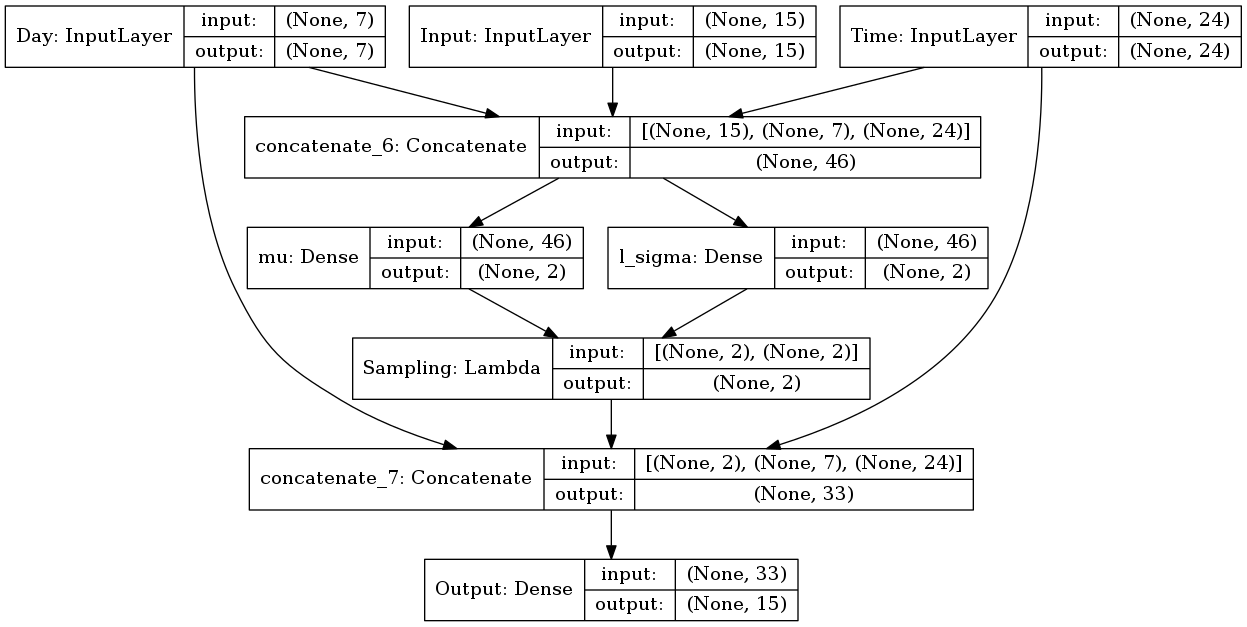
\includegraphics[width=1\textwidth]{images/c_vae}
     \caption{Schema of Conditional Variational Autoencoder}
     \label{fig:cvae_schema}
 \end{figure}
 
\subsection{Intuition}
To understand intuitively what we would expect the CVAE to accomplish, let us consider the case of learning the density distribution $P(X)$ over a dataset $X$ where each $X$ has a label $y$ for each $x \in X$ that tells us explicitly what $x$ is. More specifically, let us consider the case of handwritten digits and the MNIST dataset. When training a VAE to learn the density distribution of the MNIST dataset, we would expect the encoder to learn an encoding $Q(z|X)$ that clearly delineated between the different digits. Intuitively this makes sense since in order to generate different digits the decoder has to 'decide' which digit it wants to generate before doing so. In order to be able to 'decide' which digit to generate it should have a set of points in its latent variable model that specifically allow it to choose between generating different digits. Consequently, to do so, the encoder of the VAE will learn a latent variable model where a key portion of the latent space is dedicated to offering the decoder this ability. To visualise this Figure \ref{fig:mnist_vae} shows the latent space of a VAE with an encoder/decoder architecture composed of one intermediate encoding/decoding layer of 512 neurons. \\

\begin{figure}[htbp]
    \centering
    \includegraphics[width=1\textwidth]{images/MNIST_VAE}
    \caption{VAE MNIST latent space}
    \label{fig:mnist_vae}
\end{figure}

The plot of the latent space clearly illustrates that indeed the encoder learns to delineate between the different digits to be generated, and intuitively this makes sense as generating digits is first and foremost the task of the VAE. Secondary concerns would be learning the nuances of how to generate digits. To be able to do so however, the VAE would have to be relieved of the task of learning the differences between digits and allowed to fully emphasise learning the nuances of each digit. The way this is accomplished is by training a Conditional Variational Autoencoder that is conditioned on the digit to be generated. To visualise this, a CVAE of a similar architecture is trained as the VAE above with the exception that it is now conditioned on a one-hot vector of the specific digit being encoded and decoded. The latent space encoding is visualised in Figure \ref{fig:mnist_cvae}. \\

\begin{figure}[htbp]
    \centering
    \includegraphics[width=1\textwidth]{images/MNIST_CVAE}
    \caption{CVAE MNIST latent space}
    \label{fig:mnist_cvae}
\end{figure}

In Figure \ref{fig:mnist_cvae} we observe clearly that the encoding space no longer delineates between the different digits to be generated. Instead, the points are homogeneously distributed around the centre according to the prior $P(z)$. In fact, for each value the conditional variable $c$ can take on, the CVAE learns a specific distribution of the points associated with that condition. When generating images from latent variables, by sampling points uniformly across the latent space and decoding them the VAE generates different digits across the latent space whereas the CVAE will generate the same digit with different forms when points are sampled across the latent space and conditioned on a random variable $c$. The results are visualised in Figures \ref{fig:mnist_decode} and \ref{fig:cmnist_decode}. In what follows we test conditioning the CVAE on the time \& day an activity vector occurs as well as conditioning the CVAE on a summary of the activities that preceded the activity vector being encoded/decoded. To test the degree of control over the generative process the different conditional variables possess the latent space encoding conditioned on $c$ will be compared to Figure \ref{fig:mnist_cvae}. Conditional latent variables that result in a near-homogeneous mixing of points centred around the origin will prove to be powerful conditional variables that allow the CVAE to prioritise less learning to reconstruct individual apps and shift towards learning the nuances of how activity vectors are structured, akin to how in the case of MNIST the CVAE is able to learn how different digits are generated instead of learning how to generate different digits. 

\begin{figure}[htbp]
    \centering
    \includegraphics[width=0.5\textwidth]{images/VAE_MNIST_Decode}
    \caption{MNIST images generated by sampling uniformly from VAE latent space}
    \label{fig:mnist_decode}
\end{figure}

\begin{figure}[htbp]
    \centering
    \includegraphics[width=0.5\textwidth]{images/CVAE_MNIST_Decode}
    \caption{MNIST images generated by sampling uniformly from CVAE latent space with c=5}
    \label{fig:cmnist_decode}
\end{figure}

\subsection{Condition on Time \& Day}

Figure \ref{fig:cvae_latent} plots the latent space of the CVAE conditioned on time and day. Here, we observe that the sparsity plaguing the VAE is remarkable less prevalent and in fact the CVAE does a better job at learning the dependency between apps without compromising on reconstruction quality, as can be seen from the losses in Figure \ref{fig:cvae_loss}. Despite the smoother distribution of points across the latent space, the distribution of points in the latent space is still characterised by a clear clustering of points dominated by a single app. While a clear separation of components is definitely a desirable property of any encoding mechanism, in the case of the CVAE this implies the conditional variable $c$ does not contain enough information to allow the VAE's encoder some leniency away from encoding for the apps. In other words, in an ideal case, if the variable $c$ the CVAE is conditioning on contains \textit{enough information} to allow the decoder to reconstruct which apps are being focused on, then the CVAE would not need to partition the latent space according to clusters of apps. More specifically, if the conditional variable $c$ does contain enough information to allow reconstruction of the point being encoded then we would expect to see points in the latent space $Q(z|X,c)$ distributed as if each cluster were a normal distribution $\mathcal{N}(0,1)$ on its own! To illustrate this point

 \begin{figure}[htbp]
     \centering
     \includegraphics[width=1\textwidth]{images/VAE_TD_Latent_Space}
     \caption{Latent Space of CVAE conditioned on Hour \& Day}
     \label{fig:cvae_latent}
 \end{figure}

 \begin{figure}[htbp]
     \centering
     \includegraphics[width=1\textwidth]{images/C_VAE_Losses}
     \caption{Training \& test loss on CVAE conditioned on time \& day}
     \label{fig:cvae_loss}
 \end{figure}


 \subsection{Condition on Previous Activity}
 \begin{figure}[htbp]
     \centering
     \includegraphics[width=1\textwidth]{images/C_VAE_Prev_Latent_Space}
     \caption{Latent space of CVAE conditioned on previous activity}
     \label{fig:prev_cvae_latent}
 \end{figure}

 \begin{figure}[htbp]
     \centering
     \includegraphics[width=1\textwidth]{images/C_VAE_Losses_prev_X}
     \caption{Training \& test loss of CVAE conditioned on previous activity}
     \label{fig:prev_cvae_losses}
 \end{figure}

\section{Sampling for Prediction}
Make a prediction by reconstructing the input from time $t$ but also reconstructing the input by passing it $t+1$
 \chapter{Predictive Models} \label{predmod}
 \section{Introducing the problem}
 As previously discussed in Chapter \ref{intro}, individuals have several heuristics that guide their daily choices \citep{Kahneman1979}. These heuristics are also employed in choices of which applications to use next when accomplishing tasks or engaging in leisurely activity. This thesis hypothesizes that these mental models and frameworks can be captured by extracting patterns from observed user behaviour. More specifically, by training models that attempt to predict what applications a user will utilize next, these models will have to learn to capture these rules in order to perform well at the prediction. To test this hypothesis, this chapter explores structuring this problem as one of time-series forecasting. Assume $y_n \in \mathcal{R}^\mathcal{D} $ is an Activity Vector representing the applications a user utilized at time $n$. Given $X_n \in \mathcal{R}^{T \times \mathcal{D}}$ where $X_n$ represents the previous $T$ Activity Vectors, we would like to be able to predict $y_n$. In doing so, we make the assumption that a temporal dependency exists in a person's choice of applications, and uncovering this temporal dependency will require a class of models capable of handling sequences of data.

 \section{Sequential models}
 Neural networks have gained popularity for their successes in addressing a wide-array of pattern recognition problems ranging from optical character recognition to making diagnoses from patient medical data \citep{Amato2013}. A main shortcoming of these neural networks however is they can only handle inputs of a pre-defined size and cannot capture temporal dependencies inherent in sequential data. Better suited for handling sequential data are Recurrent Neural Networks (RNNs) and their variants the Long Short Term Memory (LSTM) \citep{Hochreiter1997} and Gated Recurrent Units (GRU) \citep{Cho2014}. RNNs have displayed state-of-the-art results in their ability to encode sequences of data into a fixed-dimensional representation vector which is then used for a myriad of tasks, such as predicting the next element in a sequence, or as input to a decoder network that generates a sequence from this encoding. The first application of RNNs, encoding a sequence into a vector representation and predicting the next sequence will be called the time-series prediction approach. The latter application of RNNs, encoding sequences into a fixed vector representation from which a decoder is initialised is commonly known as sequence-to-sequence learning. Examples of time-series prediction can be found in language modelling where RNNs are used to predict the next character or word in a sequence \citep{mikolov2010recurrent}, text generation \citep{ICML2011Sutskever_524} and stock price prediction \citep{bernal2012financial} among many others. Sequence-to-sequence Encoder-Decoder models have enjoyed huge successes in machine translation \citep{sutskever2014sequence, bahdanau2014neural} and speech recognition \citep{chan2015listen}. The Encoder-Decoder architecture has been applied to other sequence problems, such as image captioning \citep{xu2015show}, activity understanding and video captioning \citep{donahue2015long}. In encoding inputs such as images and videos, the Convolutional Neural Network (CNN) has been used due to its ability to capture both temporal and spatial dependencies. In the case of sequences that do not contain any spatial dependencies, such as a sequence of words, a 1-dimensional CNN can alternatively be used that performs convolutions only across the time dimension. These variants of the CNN have been leveraged in designing completely convolutional encoders and decoders for sequence-to-sequence learning, particularly in machine translation, where they have delivered superior accuracy results as well as offering substantial speed-ups in time required to train due to their heavily parallelizable structure \citep{gehring2017convolutional}.\\

 In the following sections, we offer a brief overview of the theory behind Recurrent Neural Networks and Convolutional Neural Networks, followed by the results of applying these models to the task of predicting future app usage and a discussion on the results.

 \section{Results \& discussion}

 % \begin{figure}[htbp]
 %   \centering
 %   \caption{2D Embedding of Conv1D predictions}
 %   \label{top_cats}
 %   \includesvg[width=1\textwidth]{images/VAE-Conv1D-Y-Pred}
 % \end{figure}

 % \begin{figure}[htbp]
 %   \centering
 %   \caption{2D Embedding of LSTM predictions}
 %   \label{top_cats}
 %   \includesvg[width=1\textwidth]{images/VAE-LSTM-Y-Pred}
 % \end{figure}

 % \begin{figure}[htbp]
 %   \centering
 %   \caption{2D Embedding of true values}
 %   \label{top_cats}
 %   \includesvg[width=1\textwidth]{images/VAE-Y-True}
 % \end{figure}

 \subsection{LSTM}
 \subsubsection{Choice of hyperparameters}

 \subsection{CNN}
 \subsubsection{Choice of hyperparameters}
 \subsection{LSTM conditioned on Time \& Day}
 \subsubsection{Choice of hyperparameters}
 \subsection{CNN condition on Time \& Day}
 \subsubsection{Choice of hyperparameters}

\chapter{Results \& Discussion} \label{res}
\chapter{Conclusions} \label{conc}

%now enable appendix numbering format and include any appendices
\appendix
\include{appendix1}
\include{appendix2}

%next line adds the Bibliography to the contents page
\bibliography{ref}        %use a bibtex bibliography file refs.bib
\bibliographystyle{plainnat}  %use the plain bibliography style
%uncomment next line to change bibliography name to references
%\renewcommand{\bibname}{References}


\end{document}